Primero y siguiendo con el orden de los Datasets mostrados serán presentados los \hyperref[fig:imagen6]{resultados} referentes a los casos limite y luego como aumentan los tiempos de ejecución respecto al aumento de caracteres, haciendo un análisis de lo que reflejan en temas de optimización y calidad de respuestas:\\

\begin{table}[h!]
    \centering
    \begin{tabular}{|c|c|c|}
    \hline
    Caso Particular & Tiempo Fuerza bruta & Tiempo Prog. Dinámica \\ \hline
    Cadenas Vacías         & 100 [ms]     & 179 [ms]    \\ \hline
    Caracteres Repetidos   & 258936 [ms]  & 5187 [ms]   \\ \hline
    Cadenas Simétricas     & 261545 [ms]  & 7075 [ms]   \\ \hline
    Cadenas Asimétricas    & 1889464 [ms] & 9615 [ms]   \\ \hline
    Matrices Iguales       & 257996 [ms]  & 6824 [ms]   \\ \hline
    \end{tabular}
    \caption{Resultados Casos Limites.}
    \label{tab:resultados1}
\end{table}

\begin{figure}[h!]
    \centering
    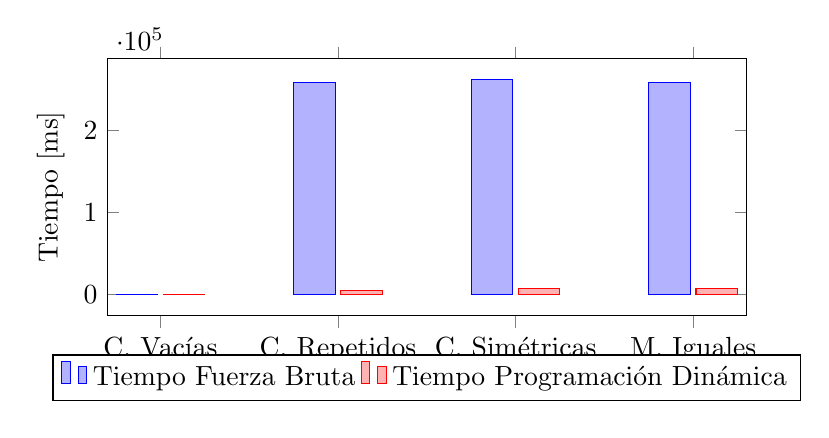
\begin{tikzpicture}
        \begin{axis}[
            ybar=2pt,
            bar width=15pt,
            xtick={1,2,3,4},
            xticklabels={C. Vacías, C. Repetidos, C. Simétricas, M. Iguales},
            ylabel={Tiempo [ms]},
            xlabel={Caso Particular}, 
            legend style={at={(0.5,-0.15)},anchor=north,legend columns=2}, 
            width=0.8\textwidth,
            height=0.4\textwidth
        ]
            \addplot coordinates {(1,100) (2,258936) (3,261545) (4,257996)};
            \addplot coordinates {(1,179) (2,5187) (3,7075) (4,6824)};
            \legend{Tiempo Fuerza Bruta, Tiempo Programación Dinámica} 
        \end{axis}
    \end{tikzpicture}
    \caption{Comparación de los tiempos de Fuerza Bruta y Programación Dinámica.}
\end{figure}

Resulta importante destacar de este gráfico que han sido quitados los valores para el caso de \textbf{Cadenas Asimétricas} ya que para el enfoque de Fuerza Bruta, como se puede ver en la Tabla, este se escapaba por mucho de los otros valores, haciendo que fuera difícil visualizarlo junto a los demás.\\

De esto es posible ver como las cadenas asimétricas no afectan en gran medida pues están directamente relacionadas a la cadena de mayor tamaño mas que al contenido de las mismas. También se puede apreciar como con cadenas vacías el enfoque de Fuerza Bruta es levemente mejor al ser más directo. Además, se ve que dentro del enfoque de Programación Dinámica la repetición de caracteres ayuda a agilizar los procesos y por último, que las matrices iguales ayudan un poco pero no significativamente al procesado de los datos y a la eficiencia de los algoritmos.

\begin{table}[h!]
    \centering
    \begin{tabular}{|c|c|c|}
    \hline
    Número Caracteres & Tiempo Fuerza bruta & Tiempo Prog. Dinámica \\ \hline
    1    &  419 [ms]        & 599 [ms]     \\ \hline
    2    &  2065 [ms]       & 1562 [ms]    \\ \hline
    3    &  9582 [ms]       & 2223 [ms]    \\ \hline
    4    &  40931 [ms]      & 3444 [ms]    \\ \hline
    5    &  257123 [ms]     & 5434 [ms]    \\ \hline
    6    &  1150738 [ms]    & 7507  [ms]   \\ \hline
    7    &  6921528 [ms]    & 9456 [ms]    \\ \hline
    8    &  26891156 [ms]   & 12050 [ms]   \\ \hline
    9    &  80437376 [ms]   & 15315 [ms]   \\ \hline
    10   &  Indefinido      & 18769 [ms]   \\ \hline
    \end{tabular}
    \caption{Resultados Aumento Progresivo de Caracteres.}
    \label{tab:resultados2}
\end{table}

\begin{figure}[h!]
    \centering
    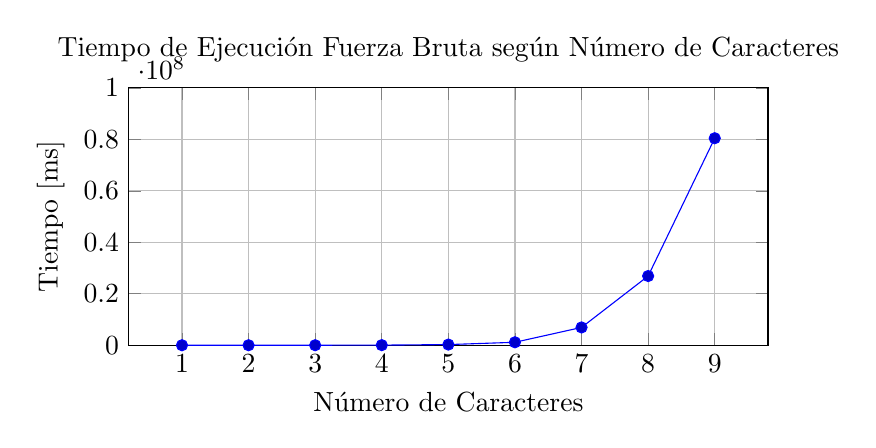
\begin{tikzpicture}
        \begin{axis}[
            xlabel={Número de Caracteres},
            ylabel={Tiempo [ms]},
            title={Tiempo de Ejecución Fuerza Bruta según Número de Caracteres},
            grid=both,
            ymin=0, ymax=100000000,
            ytick={0,20000000,40000000,60000000,80000000,100000000},
            xtick={1,2,3,4,5,6,7,8,9}, 
            width=0.8\textwidth, 
            height=0.4\textwidth,
            legend style={at={(0.5,-0.15)},anchor=north}
        ]
            \addplot coordinates {(1,419) (2,2065) (3,9582) (4,40931) (5,257123) (6,1150738) (7,6921528) (8,26891156) (9,80437376)};
        \end{axis}
    \end{tikzpicture}
\end{figure}

\begin{figure}[h!]
    \centering
    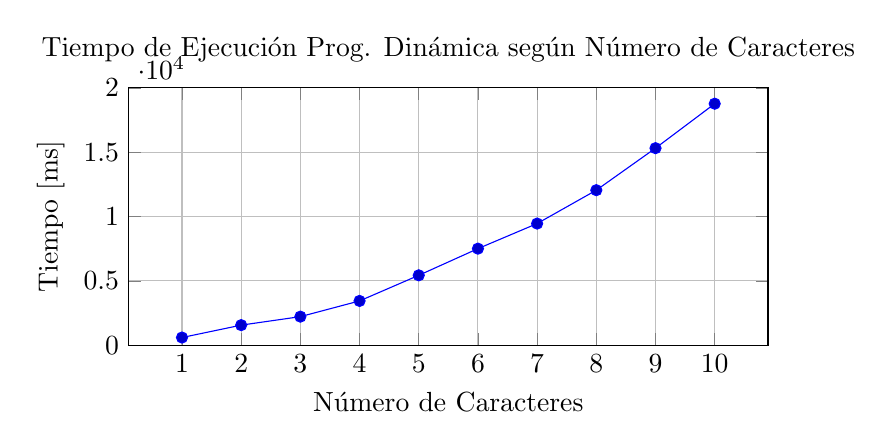
\begin{tikzpicture}
        \begin{axis}[
            xlabel={Número de Caracteres},
            ylabel={Tiempo [ms]},
            title={Tiempo de Ejecución Prog. Dinámica según Número de Caracteres},
            grid=both,
            ymin=0, ymax=20000,
            ytick={0,5000,10000,15000,20000},
            xtick={1,2,3,4,5,6,7,8,9,10}, 
            width=0.8\textwidth, 
            height=0.4\textwidth,
            legend style={at={(0.5,-0.15)},anchor=north}
        ]
            \addplot coordinates {(1,599) (2,1562) (3,2223) (4,3444) (5,5434) (6,7507) (7,9456) (8,12050) (9,15315) (10,18769)};
        \end{axis}
    \end{tikzpicture}
\end{figure}

\newpage
\subsection{Análisis de Resultados}

Es posible ver para la \textbf{Fuerza Bruta} que a medida que incrementa el número de caracteres en las cadenas de entrada, la cantidad de llamadas recursivas y los subproblemas a resolver aumenta drásticamente, lo que provoca una crecimiento exponencial del tiempo de ejecución. En experimentos prácticos, se observa que, para cadenas de longitud moderada, el tiempo de ejecución aumenta significativamente, y se vuelve inviable para cadenas más largas (por ejemplo, más de 10-12 caracteres). Esto se debe a que el número de subproblemas crece exponencialmente con el tamaño de las cadenas, lo que hace que el algoritmo sea muy lento.\\

La \textbf{Programación Dinámica} mejora considerablemente la eficiencia del algoritmo, ya que solo resuelve cada subproblema una vez. Este enfoque es significativamente más rápido en comparación con la fuerza bruta, especialmente cuando las cadenas tienen longitudes mayores. Los resultados experimentales muestran que no se ve significativamente afectado, el algoritmo de Programación Dinámica es mucho más rápido y sigue siendo manejable en términos de tiempo de ejecución.\\

En el caso de cadenas simétricas, el algoritmo de Fuerza Bruta sigue siendo relativamente lento y peor que el de Programación Dinámica, ya que evalúa todas las combinaciones posibles de operaciones. Sin embargo, debido a la regularidad de la estructura de las cadenas, el número de subproblemas realmente distintos a resolver puede ser menor, lo que reduce parcialmente el tiempo de ejecución. Por otro lado, en el caso de cadenas asimétricas, la Fuerza Bruta se ve seriamente afectada. Debido a la falta de regularidad en la estructura de las cadenas, el número de subproblemas a resolver crece de manera exponencial. El único caso en el que es mejor un enfoque de Fuerza Bruta es en el de cadenas vacías y se debe a la simplicidad del mismo.\\
